\chapter{Supported Measurement Corrections}
\label{chap:corrections}
There are a number of corrections implemented in SALSA which may be used to modify the measurement data of the user.  For convenience, we have tabulated which corrections apply to which record types in the Table \ref{tab:corrections}.
\begin{table}[!htbp]
\centering
\begin{tabular}{|l|c|c|c|c|c|c|c|c|c|c|}\hline
\tiny{\textbf{Record Type}}&\tiny{\textbf{Curv}}&\tiny{\textbf{Hgt}}&\tiny{\textbf{Reduced}}&\tiny{\textbf{Refract}}&\tiny{\textbf{OHC}}\\\hline
\tiny{\textbf{AZIM}}&&\tiny{\textbf{X}}&\tiny{\textbf{X}}&&\\\hline
\tiny{\textbf{DIST}}&&\tiny{\textbf{X}}&&&\\\hline
\tiny{\textbf{DXYZ}}&&\tiny{\textbf{X}}&&&\\\hline
\tiny{\textbf{HANG}}&&\tiny{\textbf{X}}&\tiny{\textbf{X}}&&\\\hline
\tiny{\textbf{HDIF}}&\tiny{\textbf{X}}&&\tiny{\textbf{X}}&\tiny{\textbf{X}}&\tiny{\textbf{X}}\\\hline
\tiny{\textbf{VANG}}&&\tiny{\textbf{X}}&\tiny{\textbf{X}}&\tiny{\textbf{X}}&\\\hline
\tiny{\textbf{ZANG}}&&\tiny{\textbf{X}}&\tiny{\textbf{X}}&\tiny{\textbf{X}}&\\\hline
\end{tabular}
\caption{Table indicating which types of corrections may be applied to which type of record.}
\label{tab:corrections}
\end{table}
\section{Measurement Records}
\subsection{AZIM: Azimuthal Angles} \label{subsection:AZIM}
The azimuth angle record between two points is nominally defined as
\begin{equation}
\text{AZIM} = \underbrace{\f{\pi}{2}-\tan^{-1}\left(\f{\Delta N}{\Delta E}\right)}_{\text{Nominal}}+\text{Corr}_{\text{Hgt}}+\text{Corr}_{\text{DoV}}.
\end{equation}
We have denoted the northernly displacement by $\Delta N$ and the eastwardly displacement by $\Delta E$.
\subsection{DIST: Distance Measurement} \label{subsection:DIST}
The distance measurement is nominally computed as the Pythagorean distance between the two points
\begin{equation}
\text{DIST} = \underbrace{\sqrt{\left(X_{\text{To}}-X_{\text{From}}\right)^2+\left(Y_{\text{To}}-Y_{\text{From}}\right)^2+\left(Z_{\text{To}}-Z_{\text{From}}\right)^2}}_{\text{Nominal}}\times\text{Corr}_{\text{\text{Hgt}}}.
\end{equation}
\subsection{DXYZ: 3-D XYZ Coordinate Difference} \label{subsection:DXYZ}
In ECEF XYZ coordinates, the difference in coordinates is nominally given as
\begin{equation}
\text{DXYZ}=\left(\begin{array}{c}\Delta X\\\Delta Y\\\Delta Z\end{array}\right) = \underbrace{\left(\begin{array}{c}\left(X_{\text{To}}-X_{\text{From}}\right)\\\left(Y_{\text{To}}-Y_{\text{From}}\right)\\\left(Z_{\text{To}}-Z_{\text{From}}\right)\end{array}\right)}_{\text{Nominal}}+\left(\begin{array}{c}\text{Corr}_{\text{Hgt},X}\\\text{Corr}_{\text{Hgt},Y}\\\text{Corr}_{\text{Hgt},Z}\end{array}\right).
\end{equation}
\subsection{HANG: Horizontal Angle}
The horizontal angle between two points may be nominally rewritten (see Figure \ref{Fig:HANG}) as the difference in azimuthal angles between those two points as follows,
\begin{equation}
\text{HANG}=\underbrace{\left(\text{AZIM}_{\text{To,At}}-\text{AZIM}_{\text{From,At}}\right)}_{\text{Nominal}}+\text{Corr}_{\text{Hgt}}+\text{Corr}_{\text{DoV}}.
\end{equation}
\begin{figure}[!htbp]
\centering
\begin{tikzpicture}
\draw (-0.1,-0.1) node{{\color{blue}{\tiny{\textbf{At}}}}};

\draw[straight,color=black,line width=0.25mm] (0,0) -- (0,2);
\draw[straight,color=black,line width=0.25mm,dashed] (0,0) -- (2,2*1.414) node{{\color{blue}{\tiny{\textbf{From}}}}};
\draw[straight,color=black,line width=0.25mm,dashed] (0,0) -- (2*1.414,2) node{{\color{blue}{\tiny{\textbf{ To}}}}};
\draw[color=red,line width=0.25mm,dashed] (0,0.5) arc (90:80:1.8);
\draw[color=red,line width=0.25mm,dashed] (0,1.5) arc (90:45:1.8);
\draw[color=blue,line width=0.25mm,dashed] (1.4,1.9) arc (80:55:1.8);
\end{tikzpicture}
\caption{Horizontal angle measurements may be thought of as the difference of two azimuthal angle measurements.}
\label{Fig:HANG}
\end{figure}
\subsection{HDIF: Height Difference} \label{subsection:HDIF}
The difference in ellipsoidal heights is nominally given as
\begin{eqnarray*}
\text{HDIF} &=& \underbrace{\left(h_{\text{To}}-h_{\text{From}}\right)}_{\text{Nominal}}\\
&=&\left(H_{\text{To}}-H_{\text{From}}\right)+\left[\left(\text{Geoid Height}\right)_{\text{To}}-\left(\text{Geoid Height}\right)_{\text{From}}\right]\\
&& + \text{Corr}_{\text{Curv}} + \text{Corr}_{\text{Reduced}} + \text{Corr}_{\text{Refrac}} + \text{Corr}_{\text{OHC}}.
\end{eqnarray*}
By default, it is assumed that the user has input an orthometric height difference.
\subsection{VANG: Vertical Angle} \label{subsection:VANG}
The vertical angle is given trigonometrically (see Figure \ref{Fig:VANG}) by
\begin{equation}
\text{VANG} =\underbrace{\sin^{-1}\left(\f{\Delta U}{D}\right)}_{\text{Nominal}}+\text{Corr}_{\text{Hgt}}+\text{Corr}_{\text{DoV}}+\text{Corr}_{\text{Refrac}}.
\end{equation}
Here $\Delta U$ denotes the up displacement between the ``To'' site and the ``From'' site.  The Pythagorean slant distance is denoted by $D$.
\begin{figure}[!htbp]
\centering
\begin{tikzpicture}
\draw (1,1.4) node{{\color{blue}{\tiny{\textbf{D}}}}};
\draw (2.6,1) node{{\color{blue}{\tiny{$\mathbf{\Delta}$\textbf{U}}}}};
\draw (0.5,0.2) node{{\color{blue}{\tiny{$\theta$}}}};

\draw[straight,color=black,line width=0.25mm] (0,0) -- (2,0);
\draw[straight,color=black,line width=0.25mm] (0,0) -- (0,2);
\draw[straight,color=blue,line width=0.25mm,dashed] (0,0) -- (2,2);
\draw[straight,color=blue,line width=0.25mm,dashed] (2,0) -- (2,2);
\end{tikzpicture}
\caption{The vertical angle is trigonometrically related to the upwardly displacement $\Delta U$ and the Pythagorean slant distance $D$.}
\label{Fig:VANG}
\end{figure}
\subsection{ZANG: Zenith Angle}
The zenith angle is the complement angle to the vertical elevation angle.  Therefore we obtain
\begin{equation}
\sin\left(\text{VANG}\right)=\sin\left(\f{\pi}{2}-\text{ZANG}\right)=\cos\left(\text{ZANG}\right).
\end{equation}
This results in 
\begin{equation}
\text{ZANG}=\underbrace{\cos^{-1}\left(\f{\Delta U}{D}\right)}_{\text{Nominal}}+\text{Corr}_{\text{Hgt}}+\text{Corr}_{\text{DoV}}+\text{Corr}_{\text{Refrac}}.
\end{equation}
\section{Curvature}
In this section we will discuss the curvature correction.  This correction is enabled by default, but if your instrument is configured to perform the corrections itself this option should be disabled.
\subsection{HDIF: Height Difference}
When this option is applied to HDIF records, the height difference arising from the curvature of the Earth is approximated and removed.  Begin by noting that the geometry of the problem displayed in Figure \ref{Fig:Curv} implies the following relationship (utilizing the small angle approximation)
\begin{equation}
\alpha \approx \f{\Delta H}{D} \approx \f{(D/2)}{R_{\text{Earth}}}.
\end{equation}

\begin{figure}[!htbp]
\centering
\begin{tikzpicture}
\draw (-1.,2) node{{\color{blue}{\tiny{\textbf{$R_{\text{Earth}}$}}}}};
\draw (0.5,2) node{{\color{blue}{\tiny{\textbf{$R_{\text{Earth}}$}}}}};
\draw (-1.,3.8) node{{\color{blue}{\tiny{\textbf{$\Delta H$}}}}};
\draw (-0.32,3.65) node{{\color{blue}{\tiny{\textbf{$D$}}}}};
\draw (-0.2,2) node{{\color{blue}{\tiny{\textbf{$\alpha$}}}}};

\draw[straight,color=black,line width=0.8mm] (0,0) -- (-0.7,3.7);
\draw[straight,color=red,line width=0.25mm,dashed] (-0.7,3.7) -- (-0.7,4);
\draw[straight,color=red,line width=0.25mm,dashed] (-0.7,4) -- (0,4);
\draw[straight,color=black,line width=0.8mm] (0,0) -- (0,4);
\draw (0,4) arc (90:135:1);

\end{tikzpicture}
\caption{The curvature correction to the height difference may be directly found from geometric considerations.}
\label{Fig:Curv}
\end{figure}
We may solve this for the change in orthometric height to obtain
\begin{equation}
\text{Corr}_{\text{Curv}} = (-\Delta H) = -\f{D^2}{2R_{\text{Earth}}}.
\end{equation}
We have introduced the slant distance, $D$, which is the Pythagorean distance between the two points.  Note, one recovers (5.4) of \cite{anderson} if $R_{\text{Earth}}$ is taken to be $6371$ km.

\section{Height Corrections}
In this section we will discuss the corrections which arise due to the height of the instrument and/or the target position.
\subsection{AZIM Records}
There is a correction arising from the geodetic height of the target position.  The correction is of the form\footnote{For further details, we refer the reader to \cite{Burkholder97} or (23.33) of \cite{ghilani}.}
\begin{equation}
\text{Corr}_{\text{Hgt}}\approx\left(\f{0.108''}{1000}\right)h_{\text{To,Geodetic}}\cos^2\left(\phi_{\text{From}}\right)\sin\left(2\cdot\text{AZIM}_{\text{To,From}}\right).
\end{equation}

\subsection{DIST Records} \label{subsection:DIST_HeightCorrection}
When this option is applied to DIST records, the contribution to the distance from the instrument and target height is removed.  The general strategy is to reduce the measurement to the ellipsoid and then to recompute the slant distance.  The resulting form of the correction is \cite{Ghilani_dist_reduced}.
\begin{equation}\label{eq:dist_hgt}
\text{Corr}_{\text{Hgt}}=\sqrt{\left[1-\left(\f{h_{2,\text{tot}}-h_{1,\text{tot}}}{\text{Nominal}}\right)^2\right]\f{\left(R_{\text{Earth}}+h_2\right)\left(R_{\text{Earth}}+h_1\right)}{\left(R_{\text{Earth}}+h_{2,\text{tot}}\right)\left(R_{\text{Earth}}+h_{1,\text{tot}}\right)}+\left(\f{h_2-h_1}{\text{Nominal}}\right)^2}.
\end{equation}
We have let $h_{1,\text{tot}}$ and $h_{2,\text{tot}}$ denote the sum of the ellipsoidal height and the height offset at that point.

To easily derive this result, consider the geometry presented in Figure \ref{Fig:triangles}.

\begin{figure}[!htbp]
\centering
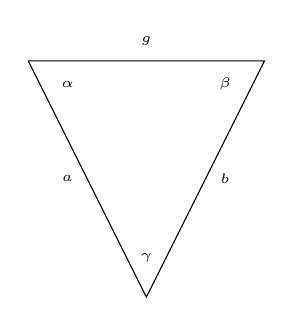
\begin{tikzpicture}
\draw (0,3)--(3,3)--(1.5,0)--(0,3);
\draw (0.5,2.7) node{{\color{black}{\tiny{\textbf{$\alpha$}}}}};
\draw (2.5,2.7) node{{\color{black}{\tiny{\textbf{$\beta$}}}}};
\draw (1.5,0.5) node{{\color{black}{\tiny{\textbf{$\gamma$}}}}};
\draw (1.5,3.25) node{{\color{black}{\tiny{\textbf{$g$}}}}};
\draw (0.5,1.5) node{{\color{black}{\tiny{\textbf{$a$}}}}};
\draw (2.5,1.5) node{{\color{black}{\tiny{\textbf{$b$}}}}};
\end{tikzpicture}~~~~~~~~~~
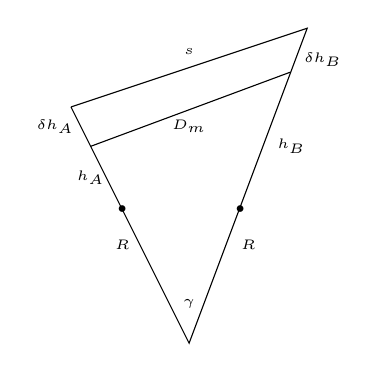
\begin{tikzpicture}
\draw (0,3)--(3,4)--(1.5,0)--(0,3);
\draw (0.25,2.5)--(2.78,3.44);
\draw (1.5,0.5) node{{\color{black}{\tiny{\textbf{$\gamma$}}}}};
\draw (1.5,3.71) node{{\color{black}{\tiny{\textbf{$s$}}}}};
\draw (1.5,2.75) node{{\color{black}{\tiny{\textbf{$D_m$}}}}};
\draw (0.65,1.7) node{{\color{black}{\tiny{\textbf{$\bullet$}}}}};
\draw (2.15,1.7) node{{\color{black}{\tiny{\textbf{$\bullet$}}}}};
\draw (0.65,1.25) node{{\color{black}{\tiny{\textbf{$R$}}}}};
\draw (2.25,1.25) node{{\color{black}{\tiny{\textbf{$R$}}}}};
\draw (0.25,2.1) node{{\color{black}{\tiny{\textbf{$h_A$}}}}};
\draw (2.8,2.5) node{{\color{black}{\tiny{\textbf{$h_B$}}}}};
\draw (-0.2,2.75) node{{\color{black}{\tiny{\textbf{$\delta h_{A}$}}}}};
\draw (3.2,3.6) node{{\color{black}{\tiny{\textbf{$\delta h_{B}$}}}}};
\end{tikzpicture}
\caption{Geometry relevant for law of cosines discussion (left) and for height correction derivation (right).  We have used $s$ to denote the nominal slant distance and $D_m$ to denote the mark-to-mark distance.}
\label{Fig:triangles}
\end{figure}
Recall that the law of cosines may be written as
\begin{equation}
g^2=a^2+b^2-2ab\cos\gamma = (a-b)^2+4ab\sin\f{\gamma}{2}.
\end{equation}
Applying the law of cosines to the geometry relevant for the correction yields
\begin{eqnarray}
s^2 = (h_{B,\text{tot}}-h_{A,\text{tot}})^2+4(R+h_{A,\text{tot}})(R+h_{B,\text{tot}})\sin\f{\gamma}{2},\\
D_m^2 = (h_{B}-h_{A})^2+4(R+h_{A})(R+h_{B})\sin\f{\gamma}{2}.
\end{eqnarray}
Combining these results yields
\begin{equation}
D_m^2 = \left(s^2-(h_{B,\text{tot}}-h_{A,\text{tot}})^2\right)\f{(R+h_A)(R+h_B)}{(R+h_{A,\text{tot}})(R+h_{B,\text{tot}})}+(h_B-h_A)^2.
\end{equation}
Factoring out the nominal slant distance, $s$, results in equation \eqref{eq:dist_hgt}.
\subsection{DXYZ Records}
When this option is applied to DXYZ records, the XYZ coordinates at each point are adjusted for the specified heights.  The height offsets at each of the points is transformed into a height offset in XYZ coordinates by
\begin{equation}
\left[\begin{array}{c}(\Delta X)_{\text{From}}\\(\Delta Y)_{\text{From}}\\(\Delta Z)_{\text{From}}\end{array}\right]=R_{\text{ENU2XYZ},{\text{From}}}\cdot\left[\begin{array}{c}0\\0\\h_{\text{offset},\text{From}}\end{array}\right],\hspace*{4mm}\left[\begin{array}{c}(\Delta X)_{\text{To}}\\(\Delta Y)_{\text{To}}\\(\Delta Z)_{\text{To}}\end{array}\right]=R_{\text{ENU2XYZ},{\text{To}}}\cdot\left[\begin{array}{c}0\\0\\h_{\text{offset},\text{To}}\end{array}\right].
\end{equation}
The correction to the DXYZ measurement (which subtracts off the difference due to the instrument and target height offset) may be written as
\begin{equation}
\text{Corr}_{\text{Hgt},XYZ}=-\left[\begin{array}{c}\left(\Delta X\right)_{\text{To}}-\left(\Delta X\right)_{\text{From}}\\\left(\Delta Y\right)_{\text{To}}-\left(\Delta Y\right)_{\text{From}}\\\left(\Delta Z\right)_{\text{To}}-\left(\Delta Z\right)_{\text{From}}\end{array}\right].
\end{equation}
\subsection{HANG Records}
Since we have written the horizontal angle as the difference of two azimuthal angles (see Figure \ref{Fig:HANG}), the target site height correction is likewise the difference of two azimuthal corrections
\begin{equation}
\text{Corr}_{\text{Hgt}}=\left(\f{0.108''}{1000}\right)\cos^2\left(\phi_{\text{At}}\right)\left[h_{\text{To,Geodetic}}\sin\left(2\cdot\text{AZIM}_{\text{To,At}}\right)-h_{\text{From,Geodetic}}\sin\left(2\cdot\text{AZIM}_{\text{From,At}}\right)\right].
\end{equation}
\subsection{VANG Records}
The correction to the VANG measurement may be written as
\begin{equation}
\left(\text{Nominal}\right) + \text{Corr}_{\text{Hgt}}\approx\tan^{-1}\left[\tan\left(\text{Nominal}\right)-\left(\f{\Delta h_{\text{specified}}}{\text{slant distance}}\right)\right].
\end{equation}
\subsection{ZANG Records}
The corrected ZANG record is the complementary angle to the corrected VANG record,
\begin{equation}
\left(\text{Nominal}\right)+\text{Corr}_{\text{Hgt}}\approx\f{\pi}{2}-\left[\tan^{-1}\left[\tan\left(\f{\pi}{2}-\text{Nominal}\right)-\left(\f{\Delta h_{\text{specified}}}{\text{slant distance}}\right)\right]\right].
\end{equation}
\section{Reduced to Ellipsoid}
In this section we will discuss the option of reducing your measurements to the ellipsoid.  This removes all geoid-related corrections from your measurements.  This usually takes the form of preventing deflection of vertical corrections from being applied.  The two deflection of vertical components are given by
\begin{equation}
\begin{split}
\xi\hspace*{2mm}\left(\text{North--South Direction}\right)&=\Phi-\phi,\\
\eta\hspace*{2mm}\left(\text{East--West Direction}\right)&=\left(\Lambda-\lambda\right)\cos\phi.
\end{split}
\end{equation}
The symbols $\left\{\phi,\lambda\right\}$ denote the ellipsoidal latitude and longitude.  The symbols $\left\{\Phi,\Lambda\right\}$ denote the astronomical latitude and longitude.

In order to relate this to the language of North--South and East--West, consider the following:\\
$(\xi<0)$: A negative meridian component (MC) of Deflection of the Vertical (DoV) indicates that the astronomic latitude ($\Phi$) will fall to the south of the corresponding geodetic latitude ($\phi$) of the point.\\
$(\eta<0)$: A negative prime vertical component (PVC) of the Deflection of the Vertical (DoV) indicates that the astronomic longitude ($\Phi$) will fall to the west of the corresponding geodetic longitude ($\lambda$) of the point.

In SALSA, these parameters are computed by noting that
\begin{equation}
\begin{split}
\tan\hspace{1mm}\xi&=-\f{\partial\left(\text{Geoid Height}\right)}{\partial\left(\text{North}\right)}=-\f{1}{\text{R}_{\text{Earth}}}\f{\partial\left(\text{Geoid Height}\right)}{\partial\phi},\\
\tan\hspace*{1mm}\eta&=-\f{\partial\left(\text{Geoid Height}\right)}{\partial\left(\text{East}\right)}=-\f{1}{\text{R}_{\text{Earth}}\cos\left(\phi\right)}\f{\partial\left(\text{Geoid Height}\right)}{\partial\lambda}.
\end{split}
\end{equation}
Note that the final forms on the right hand side agree with equation (6.184) of \cite{torge} after noting that $\tan\hspace*{1mm}\theta\approx\theta$ for small $\theta$.

\subsection{AZIM Records}
When this option is applied to AZIM records, the deflection of vertical corrections are not included.  There are two contributions from the deflection of vertical on the azimuthal angle.  The final expression for the change in azimuthal angle is given by\footnote{We refer the user to (5--98) of \cite{wellenhof} for further details.}
\begin{equation}
\text{Corr}_{\text{DoV}}=-\eta_{\text{From}}\tan\phi_{\text{From}}-\left[\xi_{\text{From}}\sin\left(\text{AZIM}_{\text{To,From}}\right)-\eta_{\text{From}}\cos\left(\text{AZIM}_{\text{To,From}}\right)\right]\cot\left(\text{ZANG}_{\text{To,From}}\right).
\end{equation}
\subsection{HANG Records}
This prevents the deflection of vertical correction from being applied.  Since we have written the horizontal angle as the difference of two azimuthal angles (see Figure \ref{Fig:HANG}), the deflection of vertical correction is likewise the difference of two azimuthal deflection of vertical corrections.  Those corrections takes the form
\begin{equation}
\begin{split}
\text{Corr}_{\text{DoV}}&=\left\{-\left[\xi_{\text{At}}\sin\left(\text{AZIM}_{\text{To,At}}\right)-\eta_{\text{At}}\cos\left(\text{AZIM}_{\text{To,At}}\right)\right]\cot\left(\text{ZANG}_{\text{To,At}}\right)\right.\\
&\left.+\left[\xi_{\text{At}}\sin\left(\text{AZIM}_{\text{From,At}}\right)-\eta_{\text{At}}\cos\left(\text{AZIM}_{\text{From,At}}\right)\right]\cot\left(\text{ZANG}_{\text{From,At}}\right)\right\}.
\end{split}
\end{equation}
\subsection{HDIF Records}
When the this option is applied to HDIF records, the accounting for the geoid heights is removed,
\begin{equation}
\text{Corr}_{\text{Reduced}} = -\left[\left(\text{Geoid Height}\right)_{\text{To}}-\left(\text{Geoid Height}\right)_{\text{From}}\right].
\end{equation}
\subsection{VANG Records}
When this option is applied to VANG records, the deflection of vertical corrections are not included.  Those corrections take the form
\begin{equation}
\text{Corr}_{\text{DoV}}=-\left[\xi_{\text{From}}\cos\left(\text{AZIM}_{\text{To,From}}\right)+\eta_{\text{From}}\sin\left(\text{AZIM}_{\text{To,From}}\right)\right].
\end{equation}
\subsection{ZANG Records}
When this option is applied to ZANG records, the deflection of vertical corrections are not included.  Those corrections takes the form (see Figure \ref{Fig:ZANG_DOV})
\begin{equation}
\text{Corr}_{\text{DoV}}=\left[\xi_{\text{From}}\cos\left(\text{AZIM}_{\text{To,From}}\right)+\eta_{\text{From}}\sin\left(\text{AZIM}_{\text{To,From}}\right)\right].
\end{equation}
This correction agrees with (5--101) of \cite{wellenhof}.
\begin{figure}[!htbp]
\centering
\begin{tikzpicture}
\draw (0.175,0.4) node{{\color{blue}{\tiny{\textbf{$\alpha$}}}}};
\draw (1.3,0.7) node{{\color{black}{\tiny{\textbf{\rotatebox{45}{$\Delta \text{ZANG}=\xi\cos\alpha+\eta\sin\alpha$}}}}}};
\draw (1,2.2) node{{\color{blue}{\tiny{\textbf{$\eta$}}}}};
\draw (-0.2,1) node{{\color{blue}{\tiny{\textbf{$\xi$}}}}};

\draw[straight,color=blue,line width=0.25mm,dashed] (0,0) -- (0,2);
\draw[straight,color=blue,line width=0.25mm,dashed] (0,2) -- (2,2);
\draw[straight,color=black,line width=0.25mm,dashed] (0,0) -- (2,2);

\end{tikzpicture}
\caption{The deflection of vertical contribution to the zenith angle may be directly found from geometric considerations.  This is a top down view (looking down the ``Up'' axis) of how a North--South deflection and a East--West deflection result in a zenith angle contribution.}
\label{Fig:ZANG_DOV}
\end{figure}
\section{Refraction}
In this section we will discuss the refraction correction.  Physically, refraction impacts survey measurements by causing light to propagate through a different path length than is anticipated by the surveyor (light ``bends'' to a target as opposed to traveling in a straight-line).
\subsection{HDIF Records}
When this option is applied to HDIF records, vertical refraction is accounted for.  From Figure \ref{Fig:Refrac}, the geometrical relationship between the radius of curvature $r$ and the height difference is given by (utilizing the small angle approximation)
\begin{equation}
\delta \approx \f{\Delta H}{D} \approx \f{(D/2)}{r}.
\end{equation}

\begin{figure}[!htbp]
\centering
\begin{tikzpicture}
\draw (-1.,2) node{{\color{blue}{\tiny{\textbf{$r$}}}}};
\draw (0.5,2) node{{\color{blue}{\tiny{\textbf{$r$}}}}};
\draw (-1.,3.8) node{{\color{blue}{\tiny{\textbf{$\Delta H$}}}}};
\draw (-0.32,3.65) node{{\color{blue}{\tiny{\textbf{$D$}}}}};
\draw (-0.2,2) node{{\color{blue}{\tiny{\textbf{$\delta$}}}}};

\draw[straight,color=black,line width=0.8mm] (0,0) -- (-0.7,3.7);
\draw[straight,color=red,line width=0.25mm,dashed] (-0.7,3.7) -- (-0.7,4);
\draw[straight,color=red,line width=0.25mm,dashed] (-0.7,4) -- (0,4);
\draw[straight,color=black,line width=0.8mm] (0,0) -- (0,4);
\draw (0,4) arc (90:135:1);

\end{tikzpicture}
\caption{The refraction correction to the height difference may be directly found from geometric considerations.  We have used $r$ to denote the radius of curvature radius and $\delta$ to denote the refraction angle.}
\label{Fig:Refrac}
\end{figure}

We may introduce the refraction coefficient, $k=R_{\text{Earth}}/r$, and solve for the change in height to obtain
\begin{equation}
\text{Corr}_{\text{Refrac}} = (\Delta H) = k\f{D^2}{2R_{\text{Earth}}}.
\end{equation}
We have introduced the slant distance, $D$, which is the Pythagorean distance between the two points.

It is common for sources to give the equation for the combined effect of curvature and refraction.  
\begin{equation}
\begin{split}
\text{Corr}_{\text{Curv}}+\text{Corr}_{\text{Refrac}}&=\left(-1+k\right)\f{D^2}{2R_{\text{Earth}}}\\
&\approx \left(-1+0.14\right)\left(0.0785\right)(D/\text{km})^2\\
&\approx -0.0675 (D/\text{km})^2.
\end{split}
\end{equation}
The numerical values were chosen to demonstrate consistency with (5.7) of \cite{anderson}.  We emphasize that SALSA allows the user to specify the refraction coefficient $k$.

\subsection{VANG Records}
When this option is applied to VANG records, the refraction angle is subtracted from the measured angle.  As shown in Figure \ref{Fig:Refrac}, the added refraction angle may be written as
\begin{equation}
\delta \approx \f{(D/2)}{r}.
\end{equation}
Rewriting this in terms of the refraction coefficient $k=R_{\text{Earth}}/r$ immediately allows us to obtain the contribution which must be removed from the angular measurement
\begin{equation}
\text{Corr}_{\text{Refrac}}=-k\f{D}{2R_{\text{Earth}}}.
\end{equation}
This contribution agrees with (5.12b) of \cite{torge}.
\subsection{ZANG Records}
When this option is applied to ZANG records, it adds the refraction angle to the measurement.  Similarly to the VANG record, we choose to write the refraction angle in terms of the refraction coefficient to obtain
\begin{equation}
\text{Corr}_{\text{Refrac}}=k\f{D}{2R_{\text{Earth}}}.
\end{equation}

\section{Orthometric Height Correction}\label{sec:OHC}
In this section we will discuss the orthometric height correction.
\subsection{HDIF Records}
When this option is applied to HDIF records, the difference in gravitational acceleration between the two points is accounted for.  For brevity, we will use the subscript ``$1$'' in place of ``From'' and the subscript ``$2$'' in place of ``To'' in this section.  The definition of the orthometric height is the integral along the plumb line from the geoid to the surface of the gravitational acceleration divided by the mean gravitational acceleration along the plumb line,\footnote{See (3.106) of \cite{torge}.}
\begin{equation}
H=\f{1}{\bar{g}}\int_{\text{geoid}}^{\text{surface}}g\hspace*{1mm} dn.
\end{equation}
A useful difference to consider is the difference in integrals between the two points
\begin{equation}
\left(\bar{g}_2H_2-\bar{g}_1H_1\right)=\int_{\text{surface}_1}^{\text{surface}_2}g\hspace*{1mm} dn.
\end{equation}
By adding and subtracting by the appropriate factors, we may obtain the expression
\begin{equation}
(H_2-H_1)={\underbrace{\Delta n}_{\text{Leveling}}}+{\underbrace{\int_{\text{surface}_1}^{\text{surface}_2}\left(\f{g-\gamma_0^{45}}{\gamma_0^{45}}\right)dn-\left(\f{\bar{g}_2-\gamma_0^{45}}{\gamma_0^{45}}\right)H_2+\left(\f{\bar{g}_1-\gamma_0^{45}}{\gamma_0^{45}}\right)H_1}_{\text{Corr}_{\text{OHC}}}}.
\end{equation}
We have denoted the level measurement value as $\Delta n$.  The introduced constant, $\gamma_0^{45}$, is the normal gravitational acceleration evaluated on the surface of the ellipsoid and at 45 degrees latitude.  Numerically, this has a value of $\gamma_0^{45}=9.806199$ m/s$^2$.

In practice, the terms which comprise the orthometric height correction are not known.  Therefore Poincare-Prey Reduction\footnote{See section 3.5 of \cite{wellenhof}.} is often utilized to eliminate the mean gravitational acceleration from the expression
\begin{equation}
\bar{g}=g+\left(4.24\times10^{-7}\right)H/\text{s}^2.
\end{equation}

Performing elementary algebra we find the orthometric height correction to be approximately given by\footnote{We have used the Midpoint Rule approximation, $\int_{\text{surface}_1}^{\text{surface}_2}\left(\f{g-\gamma_0^{45}}{\gamma_0^{45}}\right)dn\approx\f{1}{2}\sum_i\left(\f{g_i-\gamma_0^{45}}{\gamma_0^{45}}\right)\left(H_2-H_1\right)$.}
\begin{equation}
\text{Corr}_{\text{OHC}}\approx\f{1}{2}\sum_i\left(\f{g_i-\gamma_0^{45}}{\gamma_0^{45}}\right)\left(H_2-H_1\right)+\left(\f{g_1-\gamma_0^{45}}{\gamma_0^{45}}\right)H_1-\left(\f{g_2-\gamma_0^{45}}{\gamma_0^{45}}\right)H_2-\left(4.317\times10^{-8}\right)(H_2-H_1).
\end{equation}

The gravitational accelerational acceleration usually is not known and therefore the normal gravitational acceleration is used in place of the physical gravitational acceleration,
\begin{equation}
\text{Corr}_{\text{OHC}}\approx\f{1}{2}\sum_i\left(\f{\gamma_i-\gamma_0^{45}}{\gamma_0^{45}}\right)\left(H_2-H_1\right)+\left(\f{\gamma_1-\gamma_0^{45}}{\gamma_0^{45}}\right)H_1-\left(\f{\gamma_2-\gamma_0^{45}}{\gamma_0^{45}}\right)H_2-\left(4.317\times10^{-8}\right)(H_2-H_1).
\end{equation}
The normal gravitational acceleration only depends on the latitude ($\phi$) and the ellipsoidal height ($h$) at the point.  Explicitly, the normal gravitational acceleration is given by
\begin{equation}
\begin{split}
\gamma &= \gamma_0 +\left[-\left(3.0877\times10^{-3}-4.3\times10^{-6}\sin^2\phi\right)(h/\text{km})+\left(7.2\times10^{-7}\right)(h/\text{km})^2\right]\text{m}/\text{s},\\
\gamma_0&=9.780327\left(1+5.3024\times10^{-3}\sin^2\phi-5.8\times10^{-6}\sin^2(2\phi)\right)\text{m}/\text{s}^2.
\end{split}
\end{equation}
Our final expressions agree with (4--46) of \cite{wellenhof}.

A common approximation scheme which is found in the literature is to assume:
\begin{itemize}
\item The orthometric heights are much larger than their difference: $H_2\sim H_1$.
\item The height dependent terms in the normal gravity are negligible: $\gamma\sim\gamma_0$.
\item $\gamma_0\sim9.780327\left(1+5.3024\times10^{-3}\sin^2\phi\right)\text{m}/\text{s}^2.$
\end{itemize}
This leads to
\begin{equation}\label{eq:OHCapprox}
\text{Corr}_{\text{OHC}}\approx-H_1\left(5.288\times10^{-3}\right)\left(\phi_2-\phi_1\right)\sin\left(2\phi_1\right).
\end{equation}
This agrees with equation (23.39) of \cite{ghilani} and equation (5.27) of \cite{anderson}.\footnote{The adjustment resulting from the use of the approximate form is in agreement with the results of GeoLab \cite{geolab}.}  We would like to emphasis that SALSA uses the more accurate expression which was previously introduced.
